\documentclass[../diss.tex]{subfiles}

% Possibly find a place for the contents of this

%\section{Implementation Approach} \label{sec:implmentationapproach}

% Before development could begin it was important to outline the interface to the garbage collector. The aim was to make this as familiar as the standard memory allocation functions e.g.\ \emph{malloc}/\emph{realloc}. However, the garbage collector also requires global variables which need to be initialised at the start of the program therefore extra setup functions are necessary.

% Following on from the requirements analysis, there will be an Allocator module whose role is to manage the system's memory and implement the write-barrier. A Threads module is also needed as part of the extension.

\begin{document}

This chapter will explore how the design and requirements from the previous chapter were achieved. It is discussed in seven sections: structure \& interface (\cref{sec:structureandinterface}), data structures (\cref{sec:datastructures}), the Allocator (\cref{sec:allocator}), allocating memory (\cref{sec:gcmalloc}), the Threads module (\cref{sec:threads}), garbage collection (\cref{sec:garbagecollection}), logging (\cref{sec:logger}) and implementation issues (\cref{sec:implementationissues}).

\section{Structure \& Interface}
\label{sec:structureandinterface}

In this section I will discuss the structure of the project, give a high-level overview of the garbage collector and the interface to the library.

\subsection{Directory Structure}

The project structure consists of the directory setup and build files. It is important to set these up correctly so that the codebase can remain organised and the rest of the implementation can go smoothly. The directory structure can be seen below with a description of what each contains:
\begin{itemize}
    \item benchmarks - This directory contains the benchmark source code. These benchmarks are discussed further in the evaluation.
    \item include - This contains header files which should be included by the user program to interface with the garbage collector.
    \item src - This contains the garbage collector source files.
    \item test - This directory contains the unit tests.
\end{itemize}

Each directory contains a CMakeLists.txt file since I am using CMake as my build tool. This file specifies what libraries and executables are built.

\subsection{Program Structure}

The garbage collector is composed of three modules and the public interface which ties together several parts of the program to provide garbage collection features. The interface is described in \cref{sec:interfaceoverview}, here I will give a high-level overview of the garbage collector and the key features of each part.

Figure \ref{fig:overview} shows a high-level overview of the garbage collector, which omits some subtle details which are discussed later. In the diagram a diamond represents a function, a box represents a module and arrows represent interactions between the entities. Here a module simply means part of the program which is abstracted and encapsulated therefore it can be easily replaced with alternative implementations.

\begin{figure}
    \centering
    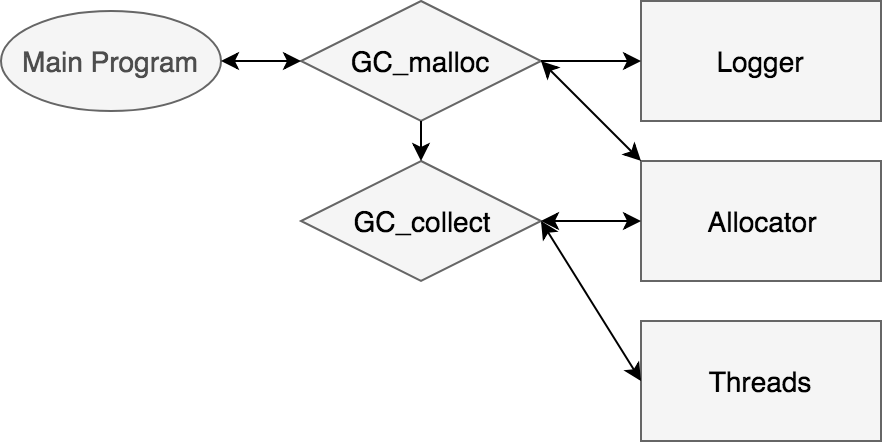
\includegraphics[max width=0.8\linewidth]{figs/overview.png}
    \caption{A high-level overview of the garbage collector}
    \label{fig:overview}
\end{figure}

The Allocator, which is discussed in \cref{sec:interfaceoverview}, is responsible for handling memory management including allocation, fragmentation and implementing a write-barrier. The write-barrier allows the Allocator to report on which objects may have been modified by the mutator since the last collection.

\emph{GC\_malloc} is how the programmer will allocate memory, it asks the Allocator for the memory and then performs some additional processing on this. When the number of allocations exceeds some threshold value, this function will call \emph{GC\_collect}. This is discussed in more depth in \cref{sec:gcmalloc}.

The Logger module is used for evaluation, it allows garbage collection statistics to be recorded which were used to produce the figures in the evaluation chapter (\cref{cpt:eval}). The logger uses the number of allocations on the x-axis, for this reason \emph{GC\_malloc} tells it to make a record each time an object is allocated. More detail is available in section \cref{sec:logger}.

The Threads module was added as part of the extension. It records information about each thread such as the location of the stack and allows communication between different threads during collection.

\emph{GC\_collect} is the main function which ties together all the functionality to perform a collection. It must be able to find the roots and perform a reachability analysis from these. It uses the Allocator to ask for modified objects since the last collection. Along with previously saved older roots it constructs the new set of older roots for dealing with cross-generational pointers. To handle multi-threaded applications I have implemented a stop-the-world collector. Signalling the threads is the responsibility of the Threads module, thus \emph{GC\_collect} first calls this signal function. Full implementation details of the \emph{GC\_collect} function can be found in \cref{sec:garbagecollection}.

\subsection{Public Interface} \label{sec:interfaceoverview}

The public interface is what the programmer will use to enable garbage collection in their project. It may be the case that the programmer wants to add this to an existing project and therefore it needs to be minimal as well as simple. Listing \ref{lst:gc.h} shows the public interface.

\begin{figure*}
\begin{lstlisting}[language=C, caption=gc.h with comments and preprocessor directives removed, label={lst:gc.h}]
void GC_init(void);
void GC_manage_thread(void);
void *GC_malloc(size_t nbytes);
void *GC_malloc_atomic(size_t nbytes);
void GC_collect(void);
void GC_stats(void);
void GC_reset (void);
\end{lstlisting}
\end{figure*}

\subsubsection{GC\_init}
This function initialises the garbage collector and as such should be called first from the main function of the user program. It also must initialise any modules which it uses such as the Allocator and Threads modules. \emph{GC\_init} makes a call to \emph{GC\_manage\_thread} to add the main thread as being managed. 

A subtlety with this function is that it uses \emph{\_\_builtin\_frame\_address} to find one endpoint of the stack. This function is compiler specific but it is defined for both GCC and Clang/LLVM compilers. So any pointers in the main function's stack frame will not be found by the garbage collector. The solution is to defer the actual work of main to another function and in main only call \emph{GC\_init} and the deferred main. An example of the problem and solution can be seen in Figure \ref{fig:stackproblem}.

\begin{figure}
    \centering
    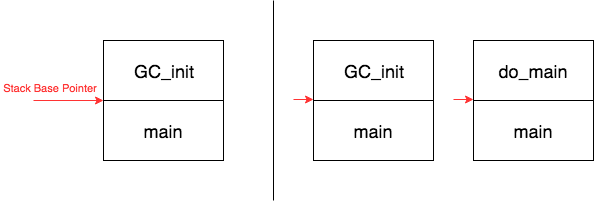
\includegraphics[max width=\linewidth]{figs/stackproblem.png}
    \caption{The inital stack frame problem}
    \label{fig:stackproblem}
\end{figure}

\begin{figure*}
\begin{lstlisting}[language=C, caption=Solution to the stack frame problem, label={lst:stackframeproblem}]
int do_main(int argc, char **argv) {
    // Do actual work
}

int main(int argc, char **argv) {
    GC_init();
    return do_main(argc, argv);
}
\end{lstlisting}
\end{figure*}

\subsubsection{GC\_manage\_thread}
This function informs the garbage collector that the current thread allocates memory that should be garbage collected. This function records the stack base pointer for each thread and therefore suffers a similar problem to \emph{GC\_init}. The solution is again to defer the actual thread work to another function.

\subsubsection{GC\_malloc}
This function is what the user program will call to allocate memory. \emph{GC\_malloc} will run the garbage collector when the number of allocations exceeds some threshold. For details on how \emph{GC\_malloc} works see \cref{sec:gcmalloc}.

\subsubsection{GC\_malloc\_atomic}
This function is analogous to \emph{GC\_malloc} with the exception that the user promises that this memory will never contain pointers to other objects. Having objects that are marked as being atomic improves performance because the garbage collector does not have to consider them as older roots.

The name, \emph{GC\_malloc\_atomic} may imply that it has something to do with concurrency. However, this is not the case and it was named after a Boehm GC method with similar functionality. This choice is for familiarity and to allow ease when switching between the two garbage collectors.

\subsubsection{GC\_collect}
Explicitly runs the garbage collector.

\subsubsection{GC\_stats}
Prints out some garbage collector statistics. Mostly used for evaluation and testing.

\subsubsection{GC\_reset}
Resets the garbage collector. Again this is used mostly for evaluation and testing.

\section{Data Structures}
\label{sec:datastructures}

The garbage collector defines many different data structures, the Allocator (\cref{sec:allocator}), Threads (\cref{sec:threads}) and Logger (\cref{sec:logger}) modules all define their own data structures which are discussed in the relevant section. Here I describe the data structures which are used in multiple parts of the program.

\subsection{GC}

This structure, which can be seen in Listing \ref{lst:gcstruct}, contains the main meta-data which the garbage collector needs. The structure contains an array of \emph{GC\_Gen} structures (\cref{sec:gcgen}) which are used to segregate the allocated objects. I also store the objects in a custom red-black tree (\cref{sec:rbtree}) which allows the garbage collector to handle modified pointers.

The roots list contains the addresses of each older root object. This list is maintained so that at any point it contains all the objects which contain pointers to other managed objects. Keeping this list up-to-date is a joint effort between the garbage collector and Allocator module.

We also keep a pointer to a \emph{logger\_t} structure which is used for collecting runtime statistics. A full description of the logger module can be found in \cref{sec:logger}.

\begin{figure*}
\begin{lstlisting}[language=C, caption=The GC structure with comments removed, label={lst:gcstruct}]
typedef struct {
    GC_Gen gen_list[GEN_COUNT];
    struct RBTree *obj_root;

    char **roots;
    unsigned int roots_size;
    unsigned int roots_count;

    logger_t *logger;

    unsigned int collections;

    unsigned int allocations;
    unsigned int frees;

    pthread_mutex_t malloc_mutex;

} GC;
\end{lstlisting}
\end{figure*}

\subsection{GC\_Gen} \label{sec:gcgen}

\emph{GC\_Gen} structures are used to segregate the allocated objects, this allows the garbage collector to traverse all objects in a particular generation without considering any other objects. This is a workaround to the problems of having a conservative collector, which were discussed in \cref{lab:conservative}. The GC\_Gen structure can be seen in Listing \ref{lst:gcgen}. 

We can have per-generation statistics for use in evaluation or testing, such as the number of collections or the number of frees. Knowing how many object are in the youngest generation is required to evaluate when the garbage collector should run.

\begin{figure*}
\begin{lstlisting}[language=C, caption=The GC\_Gen structure with comments removed, label={lst:gcgen}]
typedef struct {

    void **obj_list;
    unsigned int obj_size;
    unsigned int obj_count;

    unsigned int total_collections;

} GC_Gen;
\end{lstlisting}
\end{figure*}

\subsection{Object Headers}

It associates a header (Listing \ref{lst:gcobjheader}) with each object to store relevant meta-data. An example of this can be seen in Figure \ref{fig:objectheaders}. The advantage of this is that given a pointer to the start of the object we can quickly access the header using pointer arithmetic. Headers are added by the GC\_malloc function and the Allocator module.

The size field is used to find the bounds of each object, this is required when searching objects for internal pointers. We also have two flags: marked and atomic. Atomic objects are differentiated from non-atomic ones with a flag set to 1. The marked flag is used during the mark phase to indicate that the particular object is reachable. The current generation of the object is stored so that given an object it can easily lookup the \emph{GC\_Gen} structure which contains it.

\begin{figure}
    \centering
    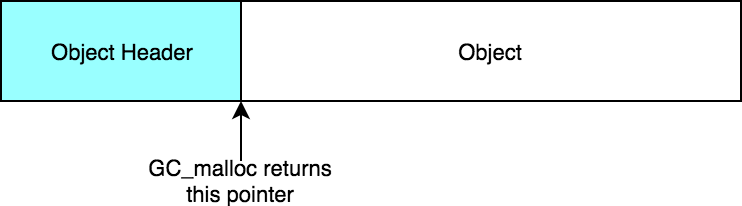
\includegraphics[max width=0.8\linewidth]{figs/objectheaders.png}
    \caption{Representation of allocated memory}
    \label{fig:objectheaders}
\end{figure}

\begin{figure*}
\begin{lstlisting}[language=C, caption=The GC\_OBJ\_H structure with comments removed, label={lst:gcobjheader}]
typedef struct {

    size_t size;
    unsigned int gen;
    unsigned int marked : 1;
    unsigned int atomic : 1;

} GC_OBJ_H;
\end{lstlisting}
\end{figure*}

\subsection{Red-Black Trees} \label{sec:rbtree}

The garbage collector makes use of a red-black tree implementation\cite{algorithms} to store pointers to all managed objects. It is used to determine whether a given pointer is pointing to an object managed by the garbage collector. We have two problems that need addressing: searching for an object should be fast and we need to handle modified pointers.

% Describe what a modified pointer is
A modified pointer is one which has been changed in some way. There are many ways to change a pointer but the red-black tree implementation is designed to handle the case when the pointer has been moved by a fixed offset. Figure \ref{fig:modifiedpointers} shows the case where a pointer has been modified in this way. Some modifications completely hide the pointers from the garbage collector such as the XORing of pointers. The user must be cautious of this as some data structures, notably the XOR linked list will cause problems for the garbage collector.


To handle modified pointers we make a change to the standard red-black tree so that our implementation uses ranges as keys. The tree property now becomes that the left subtree contains nodes whose upper keys are less than the node's lower key and similar for the right subtree. Overlapping ranges are discarded, but the garbage collector should never allocate overlapping memory so this is not a problem.

When \emph{GC\_malloc} stores an object it uses the start and end of user memory as the key and the value is a pointer to the object header. This gives us the advantage of returning the header of a miscellaneous pointer in $O(\log n)$ time.

The Allocator tends to allocate strictly increasing pointers and thus a standard binary-search tree would not be balanced leading to $O(n)$ worst case search time. I chose a red-black tree over an AVL tree because it performs fewer rotations for insertion and deletion operators which leads to better performance, despite the fact that an AVL tree is more rigidly balanced and therefore gives better search times.

\begin{figure}
    \centering
    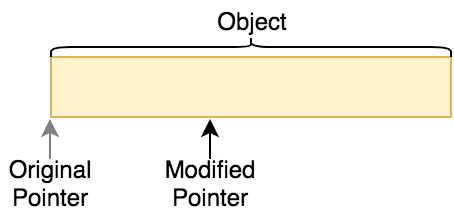
\includegraphics[max width=0.7\linewidth]{figs/modifiedpointers.png}
    \caption{Modified pointers by a fixed offset}
    \label{fig:modifiedpointers}
\end{figure}

\subsection{Lists}
Lists are a common data structure used throughout the garabge collector. Both linked lists and array lists are used where they provide the greatest performance benefit. As is good programming practice, the linked list implementation has been abstracted to provide good code reuse. However, the array list implementations are not abstracted to a separate file and reused. The reason behind this is that different array lists have slightly different behaviours, especially regarding when they expand and contract. An example of this is seen in the \emph{GC\_Gen} object where the lists shrink during collection but we do not want to contract the array as it may shortly be populated by objects promoted from a younger generation. So each array list behaves differently when needed to provide the greatest performance benefit.

\section{Allocator Module} \label{sec:allocator}

The Allocator module has several responsibilities: manage allocation and deallocation (\cref{sec:allocation}), handling fragmentation (\cref{sec:fragmentation}) and implementing a write-barrier (\cref{sec:writebarrier}). Here I will discuss how the implementation achieves these key responsibilities. Mine is one of many possibly implementations and because of good software engineering discipline the module could easily be changed in the future. Additionally, different Allocator implementations can be made to take advantage of platform-specific features and then the appropriate version can be used at compile-time. My Allocator implementation was designed to be portable and takes inspiration for the write-barrier from the Boehm GC.

\subsection{Interface \& Data Structures} \label{sec:allocatorinterface}

Listing \ref{lst:allocatorinterface} shows the allocator interface. \emph{Allocator\_alloc} and \emph{Allocator\_free} are discussed in \cref{sec:allocation} while \emph{Allocator\_dirty\_objects}, \emph{Allocator\_make\_writable} and \emph{Allocator\_clean\_all} are discussed in \cref{sec:writebarrier}. The function \emph{Allocator\_init} is called by the garbage collector during \emph{GC\_init}.

\begin{figure*}
\begin{lstlisting}[language=C, caption=The Allocator interface with comments removed, label={lst:allocatorinterface}]
void Allocator_init (void);
void *Allocator_alloc (unsigned int size);
void Allocator_dirty_objects(void (*f)(void *));
void Allocator_clean_all(void);
void Allocator_make_writable(void);
int Allocator_free (void *ptr);
\end{lstlisting}
\end{figure*}

The Allocator module creates a single instance of the \emph{Allocator\_t} structure (Listing \ref{lst:allocatorstruct}) which encapsulates a list of \emph{Page\_t} objects which are described in \cref{sec:allocation}.

\begin{figure*}
\begin{lstlisting}[language=C, caption=Allocator\_t structure with comments removed, label={lst:allocatorstruct}]
typedef struct {

    Page_t *pages;
    unsigned int page_size;
    unsigned int page_count;

} Allocator_t;
\end{lstlisting}
\end{figure*}

\subsection{Allocation \& Deallocation} \label{sec:allocation}

The garbage collector relies on the Allocator to manage the system's memory. In particular \emph{GC\_malloc} will request memory from the Allocator and \emph{GC\_collect} will tell the Allocator to reclaim memory which is garbage.

The Allocator works by reserving large blocks of memory and allocating regions within them to the user program. The reservation process (Algorithm \ref{alg:reservepage}) occurs when there is no free space large enough to allocate an object, the size of each block is the smallest multiple of the page size (typically 4KiB but this depends on the specific architecture) that is larger than the allocation amount. The reason behind this is discussed in \cref{sec:writebarrier}. Each block of memory is associated with a \emph{Page\_t} object (Listing \ref{lst:pagestruct}) which records the location and size of the block, the allocated objects stored in it and the areas of free memory. \emph{BlockRange\_t} structures (Listing \ref{lst:blockrange}) are associated with areas of free memory within a page.

\begin{figure*}
\begin{lstlisting}[language=C, caption=Page\_t structure with comments removed, label={lst:pagestruct}]
typedef struct {

    char *start_ptr;
    unsigned int page_size;
    unsigned int dirty;

    void **object_list;
    unsigned int object_count;
    unsigned int object_size;

    BlockRange_t *blocks;
    unsigned int block_size;
    unsigned int block_count;

} Page_t;

\end{lstlisting}
\end{figure*}

\begin{figure*}
\begin{lstlisting}[language=C, caption=BlockRange\_t structure with comments removed, label={lst:blockrange}]

typedef struct {

    char *start_ptr;
    unsigned int size;

} BlockRange_t;

\end{lstlisting}
\end{figure*}

The Allocator also adds a header (Listing \ref{lst:allocatorheader}) on to allocated memory which stores associated meta-data. It stores the size of each object so that it can reclaim the memory and it also stores the index of the page containing the object for fast lookup times. Storing meta-data in this way means that there is no large data-structure that needs to be maintained and pointer arithmetic can be used to lookup meta-data quickly.

\begin{figure*}
\begin{lstlisting}[language=C, caption=AllocatorObjH\_t structure with comments removed, label={lst:allocatorheader}]
typedef struct {

    unsigned int size;
    int page_index;

} AllocatorObjH_t;

\end{lstlisting}
\end{figure*}

Algorithm \ref{alg:allocation} demonstrates how the \emph{Allocator\_alloc} function works. \emph{Page\_allocate} (Algorithm \ref{alg:pageallocate}) will search through free areas of memory and if it finds space then it will reserve it for the object. When there is not enough memory the Allocator will attempt to reserve a new page of memory (Algorithm \ref{alg:reservepage}). The garbage collector allows for parts of the program to be manual memory managed so it takes control of heap memory only when necessary.

Deallocation (Algorithm \ref{alg:deallocation}) is performed by adding the memory back as a new \emph{BlockRange\_t} object. The range then gets merged with other ranges in an attempt to deal with fragmentation (\cref{sec:fragmentation}). Deallocation is made more efficient by storing the page index in the header, so that we know which page to add the range into. When an object is deallocated, the contents are invalidated by setting all the bytes to 0. This is particularly useful for evaluation as collecting a live object is more likely to result in an error.

\begin{algorithm}
\caption{Reserving Pages}
\label{alg:reservepage}
\begin{algorithmic}

\Function{reserve\_page}{$minSize$}

\State $block\_size\gets $ some multiple of the page size larger than $minSize$

\State $mem\_ptr\gets$ Allocate $block\_size$ bytes.
\State \Call{mprotect}{$mem\_ptr$, Read\&Write}

\State Add a new page to $pages$
\State Add a new block range, [$mem\_ptr$, $mem\_ptr + block\_size$] to the new page

\EndFunction

\end{algorithmic}
\end{algorithm}

\begin{algorithm}
\caption{Allocating Memory}
\label{alg:allocation}
\begin{algorithmic}

\Function{Allocator\_alloc}{$size$}

\State $allocation\_size\gets size + $ header size

\State $(obj, page)\gets $ \Call{Page\_allocate}{$allocation\_size$}
\Comment{Searches for free memory}

\If{$page$ exists}
    \State Add header to $obj$
    \State Adjust $obj$ pointer
    \State Add $obj$ to $page.obj\_list$
    \State \Return $obj$
\Else
    \State Reserve a new page and retry
\EndIf

\EndFunction

\end{algorithmic}
\end{algorithm}

\begin{algorithm}
\caption{Page\_allocate}
\label{alg:pageallocate}
\begin{algorithmic}

\Function{Page\_allocate}{$size$}

\ForAll{$page\gets pages$}

    \ForAll{$block\gets page.blocks$}
    
        \If{$block.size \geq size$}
            \State $obj\gets $Allocate memory and update $block$
            \State \Return $(obj, page)$
        \EndIf
    
    \EndFor

\EndFor

\State \Return Failed

\EndFunction

\end{algorithmic}
\end{algorithm}


\begin{algorithm}
\caption{Deallocation}
\label{alg:deallocation}
\begin{algorithmic}

\Function{Allocator\_free}{$obj$}

\State $header\gets $ \Call{get\_allocator\_header}{$obj$}
\Comment{Extract the object header}

\State $size\gets header.size$ 
\State $page\_index\gets header.page$

\State $page\gets pages[page\_index]$

\State
\State Set the memory to 0s
\State Add a new block range, $[header, header + size]$ to $page$
\State Remove $obj$ from $page.obj\_list$

\EndFunction

\end{algorithmic}
\end{algorithm}

\subsection{Fragmentation} \label{sec:fragmentation}

Fragmentation is a large problem when managing the heap. As it becomes more fragmented there is a greater chance that it will fail to allocate large amounts of memory successfully. I previously discussed why it is not possible to have a compaction function that deals with this. See \cite{fragmentation} for an overview of techniques used to deal with fragmentation.

Instead my garbage collector tries to mitigate the issues of fragmentation in two ways. Firstly, when allocating memory it tries to fill existing gaps in the page left behind by deallocated objects. Secondly, when memory is deallocated, the block ranges are merged together so that the largest possible ones remain.

Block ranges within a page have the following three invariants:
\begin{enumerate}
    \item They are sorted by start address in ascending order.
    \item They always represent the largest possible contiguous block of memory.
    \item It is impossible to have a range of 0 bytes.
\end{enumerate}

These properties are maintained with a function named \emph{BlockRange\_fixup}, which is called when the the block ranges change (during allocation or deallocation). The fixup algorithm can be seen in Algorithm \ref{alg:fragmentation}, this is broken down into three passes: Sorting, Merging and Removing 0s. The sorting pass uses insertion sort based on the assumption that block range lists tend to be small. The merge pass runs in linear time by walking along the list combining contiguous blocks. This pass produces 0s which are removed by the final pass, which also runs in linear time. This pass counts the number of removed blocks and updates the total count. Merging block ranges and removing ranges of size 0 bytes is important in keeping the list small and therefore reinforces the choice of insertion sort.

\begin{algorithm}
\caption{Handling Fragmentation}
\label{alg:fragmentation}
\begin{algorithmic}

\Function{Allocator\_alloc}{$page$}

\State \Call{Insertion\_Sort}{$page.block\_ranges$}
\Comment{Sorting Pass}

\State

\State $iMaj\gets 0$
\Comment{Merge Pass}
\State $iMin\gets iMaj + 1$

\While{$iMaj < page.block\_count$ AND $iMin < page.block\_count$}

    \State $blockMaj\gets page.block\_ranges[iMaj]$ 
    \State $blockMin\gets page.block\_ranges[iMin]$ 
    
    \State
    
    \If{$blockMaj.start\_ptr + blockMaj.size == blockMin.start\_ptr$}
        \State $blockMaj.size += blockMin.size$
        \State $blockMin.size = 0$
        \State $iMin\gets iMin + 1$
    \Else
        \State $iMaj\gets iMin$
        \State $iMin\gets iMaj + 1$
    \EndIf

\EndWhile

\State

\State $zeroCount\gets 0$
\Comment{Remove 0s Pass}

\ForAll{$block\gets page.block\_ranges$}
    \If{$block.size == 0$}
        \State Remove $block$
        \State $zeroCount\gets zeroCount + 1$
    \EndIf
\EndFor

\State $page.block\_count\gets page.block\_count - zeroCount$

\EndFunction

\end{algorithmic}
\end{algorithm}

\subsection{Write Barrier} \label{sec:writebarrier}

The write-barrier is a key part of the project as it allows me to meet the success criteria. The goal of the write-barrier is to report which objects have possibly been modified since the last collection. This works in conjunction with the rest of the garbage collector which remembers past objects that contain pointers to other objects in the global roots list (Listing \ref{lst:gcstruct}). Modified objects are checked every collection and are added to the set of older roots if they contain pointers.

The write-barrier works by making parts of the reserved memory read-only, it then traps the resultant segmentation fault and marks the page object that the write corresponds to as dirty. I previously stated that the Allocator must reserve pages (Algorithm \ref{alg:reservepage}) before allocating memory within them to the program. The write-barrier uses \emph{mprotect} to set the memory permission, this function has the condition that the amount of memory being protected is a multiple of the page size. When a page is written to, a custom signal handler is executed (Algorithm \ref{alg:wbsignal}). This makes the page writable so that future writes do not cause a segmentation fault.

The Allocator interface specifies three functions: \emph{Allocator\_dirty\_objects}, \emph{Allocator\_make\_writable} and \emph{Allocator\_clean\_all}. These are used by the collector to interact with the Allocator. Figure \ref{fig:page_lifecycle} shows how these functions affect the state of a page.

The garbage collector calls \emph{Allocator\_dirty\_objects} which takes another function as a parameter. This function is called with the address of each dirty object. The garbage collector inspects each object and merges it with the current roots set if it contains pointers to other objects. During the mark phase, objects are modified which would cause a segmentation fault if the pages were left as read-only. Especially in multi-threaded programs we do not want to enter the Allocator signal handler. So before performing any marking, the garbage collector calls \emph{Allocator\_make\_writable} which sets the permissions of every page to be read and write. After garbage collection completes, it calls \emph{Allocator\_clean\_all} which marks each page as clean and sets the permissions of each to read-only.

When a page is initially reserved it is likely that the user will write to the allocated memory. For this reason pages start their lifecycle as dirty and only become clean for the first time after the following collection. 

\begin{figure}
    \centering
    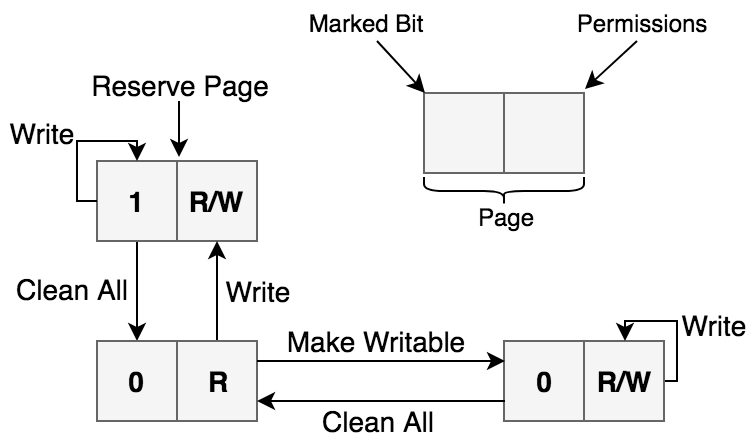
\includegraphics[max width=\linewidth]{figs/page_lifecycle.png}
    \caption{State diagram of a page}
    \label{fig:page_lifecycle}
\end{figure}

\begin{algorithm}
\caption{Write-barrier Signal Handler}
\label{alg:wbsignal}
\begin{algorithmic}

\Function{Allocator\_signal\_handler}{$signal$, $\mathit{siginfo}$}

\If{$signal$ != SIGSEGV}
\State \Return
\EndIf

\State $\mathit{fault\_loc}\gets \mathit{siginfo}.addr$

\State $page\gets$ page for location: $\mathit{fault\_loc}$
\State $page.dirty = 1$
\State \Call{mprotect}{$page$, Read\&Write}

\EndFunction

\end{algorithmic}
\end{algorithm}


\section{Allocating Memory}
\label{sec:gcmalloc}

The \emph{GC\_malloc} function is discussed in this section. A key feature of this function is that it does not perform any explicit memory management function calls but instead relies on Allocator to abstract away the lower level details. Another key feature of this function is that it must evaluate some conditions to determine if the garbage collector should run. Finally, the function should store the allocated memory in the appropriate data structures and attach an object header for meta-data.

Algorithm \ref{alg:gcmalloc}, shows how the key features outlined above are combined to produce the overall \emph{GC\_malloc} function. For thread-safety the entire function is guarded with a lock. The reason for this is that many of the function calls and data-structures are themselves not thread-safe. As a result we must restrict the order of execution to prevent unwanted behaviours. \emph{GC\_malloc\_atomic} works by simply calling \emph{GC\_malloc} and updating the atomic flag in the header.

\begin{algorithm}
\caption{Allocating Memory}
\label{alg:gcmalloc}
\begin{algorithmic}

\Function{GC\_malloc}{$size$}

\State \Call{lock}{$malloc\_mutex$}

\State $object\_count\gets gen0.obj\_count$
\Comment{Run the garabge collector}
\If{$object\_count\geq \mathit{GEN\_THRESHOLD}$}
\State \Call{GC\_collect}{\null}
\EndIf

\State
\State $obj\gets$ \Call{Allocator\_alloc}{$size+header\_size$}
\Comment{Allocate memory}

\State
\State $header\gets$ Initialise the object header
\Comment{Attach the object header}
\State Attach header to $obj$

\State
\State \Call{RBTree\_insert}{$obj\_root$, $obj$, $obj+size$, $header$}
\Comment{Update GC state}
\State Add $obj$ to generation 0

\State \Call{unlock}{$malloc\_mutex$}

\EndFunction

\end{algorithmic}
\end{algorithm}


\section{Threads Module} \label{sec:threads}

In this section I will discuss in detail the Threads module including: the interface and data structures (\cref{sec:threadsinterface}), how it manages threads (\cref{sec:threadsmanaging}), how signalling works (\cref{sec:signallingthreads}), how communication is implemented (\cref{sec:communication}) and the limits of my approach (\cref{sec:threadslimits}). Currently, my implementation uses pthreads because I am familiar with this and working on a POSIX platform. 

\subsection{Interface \& Data Structures} \label{sec:threadsinterface}

Listing \ref{lst:threadsinterface} shows the Threads interface which is how the rest of the garbage collector interacts with the module.

The Threads module defines two data structures: \emph{Thread\_t} (Listing \ref{lst:threadstruct}) and \emph{GC\_Threads\_t} (Listing \ref{lst:gcthreadsstruct}). A \emph{Thread\_t} object encapsulates data about a single thread including the \emph{pthread\_t} object which is required for signalling and the stack base pointer which allows the garbage collector to locate each stack. The \emph{GC\_Threads\_t} structure maintains a list of active threads, the condition variables required for communication and the signal handler structure. Only a single instance of the \emph{GC\_Threads\_t} object is created globally.

\begin{figure*}
\begin{lstlisting}[language=C, caption=The Threads interface, label={lst:threadsinterface}]
void Threads_init(void);
Thread_t *Threads_get_current(void);
void Threads_signal(void);
void Threads_reset(void);
void Threads_add_explicit(void *stack_base_ptr)
\end{lstlisting}
\end{figure*}

\begin{figure*}
\begin{lstlisting}[language=C, caption=The Thread\_t structure, label={lst:threadstruct}]
typedef struct {

    pthread_t tid;
    void *stack_base_ptr;

} Thread_t;
\end{lstlisting}

\begin{lstlisting}[language=C, caption=The GC\_Threads\_t structure, label={lst:gcthreadsstruct}]
typedef struct {

    Thread_t *threads;
    unsigned int thread_count;
    unsigned int thread_size;
    pthread_mutex_t threads_mutex;

    unsigned int threads_ready;
    pthread_mutex_t threads_ready_mutex;
    pthread_cond_t threads_ready_cond;

    unsigned int setup_complete;
    pthread_mutex_t threads_setup_mutex;
    pthread_cond_t threads_setup_cond;

    unsigned int threads_completed;
    pthread_cond_t threads_completed_cond;
    pthread_mutex_t threads_completed_mutex;

    unsigned int collection_completed;
    pthread_cond_t collection_completed_cond;
    pthread_mutex_t collection_completed_mutex;

    struct sigaction *threads_sig_action;
} GC_Threads_t;
\end{lstlisting}
\end{figure*}

\subsection{Managing Threads} \label{sec:threadsmanaging}

For the garbage collector to work with multi-threaded programs, it first must know that these threads exist and know some details about each one (Listing \ref{lst:threadstruct}). As such, the first task of each garbage collected thread is to call \emph{GC\_manage\_thread}. This function simply records the stack frame pointer and passes this value to \emph{Threads\_add\_explicit} (Algorithm \ref{alg:threadsaddexplicit}). Mutual exclusion is used throughout where concurrent access to shared variables can occur.

\begin{algorithm}
\caption{Recording Threads}
\label{alg:threadsaddexplicit}
\begin{algorithmic}

\Function{Threads\_add\_explicit}{$stack\_base\_ptr$}

\State $thread\gets $ \Call{pthread\_self}{\null}

\State
\State \Call{lock}{$threads\_mutex$}

\State Add a new Thread\_t($thread$, $stack\_base\_ptr$) object to $thread\_list$

\State \Call{unlock}{$threads\_mutex$}

\EndFunction

\end{algorithmic}
\end{algorithm}

This approach allows the programmer to define managed and unmanaged threads, where the unmanaged threads use manual memory management. This may be useful when the programmer knows in advance that a particular thread will not require automatic memory management features. The garbage collector will not pause execution of unmanaged threads thus the performance of these will be better when compared to the managed version.

When threads complete they must be removed from the list. Otherwise the list would only ever expand and cause a memory leak. The module uses \emph{pthread\_kill} to signal each thread at the start of a collection, this function returns a specific error code if the thread has finished. By checking the error code, it can determine whether or not a thread has finished and if so it can remove the the thread from the list. 

\subsection{Signalling Threads} \label{sec:signallingthreads}

I have implemented a stop-the-world garbage collector, which means that the main program is paused while garbage collection occurs. Collection starts when a thread making a call to \emph{GC\_malloc} triggers it, this thread becomes the collecting thread. It calls \emph{Threads\_signal} (Algorithm \ref{alg:threadsignal}) which signals every other managed thread in turn to interrupt their current execution. Every thread except for the collecting thread will enter the custom signal handler which is discussed in \cref{sec:communication}. Marking can occur in parallel safely since the only operation on shared data is to set the marked flag to 1, this is invariant in the presence of race conditions.

\begin{algorithm}
\caption{Signalling Threads}
\label{alg:threadsignal}
\begin{algorithmic}

\Function{Threads\_signal}{\null}

\State $except\gets $ \Call{pthread\_self}{\null}

\State \Call{lock}{$threads\_mutex$}

\ForAll{$thread\gets thread\_list$}

    \If{$thread$ != $except$}
        
        \State $res\gets$ \Call{pthread\_kill}{$thread$, SIGUSR1}
        \If{$res$ == Thread finished} 
            \State Remove $thread$ from $thread\_list$
        \EndIf
        
    \EndIf

\EndFor

\State \Call{unlock}{$threads\_mutex$}

\EndFunction

\end{algorithmic}
\end{algorithm}

% How we signal a thread and what the signal handler does
% Mention that this is done concurrently
% Signal handler blocks other signals

\subsection{Communication} \label{sec:communication}

As part of the garbage collection algorithm (which is discussed in \cref{sec:garbagecollection}) the collecting thread must communicate in some way with the remaining managed threads. This uses condition variables to wait on certain conditions and to signal between threads that a condition is now true. Pthread condition variables must also have an associated lock which is omitted in most algorithms for clarity, however these can be seen in Listing \ref{lst:gcthreadsstruct}. Algorithm \ref{alg:threadssignalhandler} demonstrates how the signal handler works, for details about the collecting thread, including how stack roots are found and the mark phase, see \cref{sec:garbagecollection}.

At the point of signalling, a thread it may be unable to run the signal handler immediately, this could be due to the thread being in another signal handler which cannot be preempted. The ready phase consists of the collecting thread waiting for every thread to be in the signal handler. This uses the \emph{threads\_ready} variable and the associated \emph{threads\_ready\_cond} condition variable. When the ready phase is complete, the collecting thread can perform the necessary setup to perform the collection.

Following the setup, concurrent marking between all threads occurs. Most threads consider the stack and register roots while the collecting thread also considers older roots. This choice prevents unnecessary work and still guarantees that every reachable object will be marked. The collecting thread waits for marking to be complete, which uses the \emph{threads\_completed} variable, before then performing the actual collection.

Finally, the collecting thread signals completion and waits for all other threads to exit before resetting any global values such as the condition variables for each stage.

\begin{algorithm}
\caption{Thread Signal Handler}
\label{alg:threadssignalhandler}
\begin{algorithmic}

\Function{Threads\_signal\_handler}{$signal$}

\If{$signal$ != SIGUSR1}
\State \Return
\EndIf

\State

\State \Call{lock}{$threads\_ready$} \Comment{Ready Phase}
\State $threads\_ready\gets threads\_ready + 1$
\State \Call{unlock}{$threads\_ready$}

\State

\State \Call{wait}{$setup\_complete$} \Comment{Setup Phase}

\State

\State $gen\gets$ calculate collection generation \Comment{Mark Phase}
\State $roots\gets$ new linked list
\State Place register roots on the stack
\State \Call{add\_stack\_roots}{$roots$, $gen$}
\State \Call{mark\_reachable\_objects}{$roots$, $gen$}

\State
\State $threads\_completed\gets threads\_completed + 1$
\State \Call{signal}{$threads\_completed\_cond$}

\State
\While{not $collection\_completed$}
    \State \Call{wait}{$collection\_completed\_cond$}
\EndWhile

\State

\State \Call{lock}{$threads\_ready$} \Comment{Signal Exit}
\State $threads\_ready\gets threads\_ready - 1$
\State \Call{unlock}{$threads\_ready$}

\State

\State \Call{reset\_variables}{\null}

\EndFunction

\end{algorithmic}
\end{algorithm}

\subsection{Limits} \label{sec:threadslimits}

My garbage collector uses pthreads and therefore other threading models will not be thread-safe. Also Windows machines do not have native support for pthreads and therefore requires an extension for this implementation to work correctly.

\section{Garbage Collection} \label{sec:garbagecollection}

In this section I will discuss how garbage collection was implemented. As previously mentioned in \cref{lab:conservative} we cannot implement a full copying collector and so we use a mark and sweep algorithm for every generation and have an explicit promotion phase. Algorithm \ref{alg:gc} gives the pseudo-code for the \emph{GC\_collect} function, for simplicity mutual exclusion has been omitted from the algorithm but assume that appropriate locking and unlocking is occurring. 

\begin{algorithm}
\caption{Garbage Collection}
\label{alg:gc}
\begin{algorithmic}

\Function{GC\_collect}{\null}

\State Place register roots on the stack

\State
\State \Call{Threads\_signal}{\null} \Comment{Ready Phase}
\While{$threads\_ready < thread\_count - 1$} 
    \State \Call{Wait}{$threads\_ready$}
\EndWhile

\State

\State \Call{Allocator\_dirty\_objects}{inspect\_dirty} \Comment{Setup Phase}
\State \Call{Allocator\_make\_writable}{\null}

\State

\State \Call{NotifyAll}{$setup\_complete$} \Comment{Mark Phase}

\State
\State $gen\gets $ \Call{get\_generation}{\null}
\State $roots\gets$ new linked list
\State \Call{add\_stack\_roots}{$roots$, $gen$}
\State \Call{add\_older\_roots}{$roots$, $gen$}
\State \Call{mark\_reachable\_objects}{$roots$, $gen$}

\State

\While{completed threads $<$ thread count - 1} \Comment{Wait for all threads to complete}
    \State \Call{Wait}{threads\_completed}
\EndWhile

\State
\State \Call{remove\_garbage\_roots}{$gen$}

\State
\ForAll{$generations$}
    \State Promote marked objects
    \State Collect unmarked objects
\EndFor

\State
\State \Call{Allocator\_clean\_all}{\null}

\State $collections\gets collections + 1$

\State
\State \Call{NotifyAll}{$collection\_completed$} \Comment{Signal Completion}

\While{$threads\_ready > 0$} \Comment{Wait for all threads to exit the signal handler}
    \State \Call{Wait}{$threads\_ready$}
\EndWhile

\State \Call{Threads\_reset}{\null} \Comment{Reset State}

\EndFunction

\end{algorithmic}
\end{algorithm}


\subsection{Root Finding}

% How we find roots from all the different sources including older roots
% Have a subsubsection on maintaining older roots list
It is crucial to the project that we can find pointers from the root set as well as the older objects which contain pointers. 

\subsubsection{Stack Pointers}
\label{sec:stackroots}
To search for pointers it keeps track of the start and end addresses of each stack using the function \emph{\_\_builtin\_frame\_address(0)} which returns the address of the current stack frame. As discussed in \cref{sec:threadsmanaging}, \emph{GC\_manage\_thread} will record one endpoint when called. When collecting we call this function again and search between these two pointers. This uses the assumption that the signal handler stack frame is added to the normal stack instead of a special purpose one, which may not always be true depending on the platform.

The \emph{add\_stack\_roots} function (Algorithm \ref{alg:stackroots}), uses the assumption that pointers have to be aligned on a boundary greater than or equal to the size of a pointer. It treats the entire stack as being an \emph{intptr\_t} pointer and then performs pointer arithmetic to get the values of potential references. I previously mentioned that we are using a conservative approach and therefore will get values which are in actual fact not pointers. When considering a possible pointer from the stack, it checks that it is a managed reference by performing a search in the red-black tree, this only gets added to the output list if it points to an object in a generation being collected. Objects which are not being considered for collection are ignored because if they do contain pointers they will be added when we consider older roots.

\begin{algorithm}
\caption{Finding Stack Roots}
\label{alg:stackroots}
\begin{algorithmic}

\Function{add\_stack\_roots}{$list$, $gen$}

\State $current\_thread\gets $ \Call{Threads\_get\_current}{\null}
\State $start\gets current\_thread.stack\_base\_pointer$
\State $end\gets $ \Call{\_\_builtin\_frame\_address}{0}
\State $cursor\gets start$ as intptr\_t * 

\While{$cursor < end$}
    \State $p\gets$ dereference $cursor$
    \If{$p$ is a managed pointer}
        \If{$p.gen \leq gen$}
            \State add $p$ to $list$
        \EndIf
    \EndIf
    \State $cursor\gets cursor+1$
\EndWhile

\EndFunction

\end{algorithmic}
\end{algorithm}

\subsubsection{Register Pointers}
Registers can contain pointers to heap objects which may not be on the stack. The user program could choose to keep certain pointers in registers for faster access. It is important to note that compiling with no optimisation may cause every pointer to be placed on the stack but this could possibly damage performance. 

I reused the existing stack searching code to also include registers by using the function \emph{setjmp}. \emph{setjmp} saves the current state required to restore program execution at that point, this includes saving any preserved register values. These values are stored on the stack in a platform-specific structure.

\subsubsection{Older Roots}

Finally, it must find older roots to be able to safely find all reachable objects and thus remove garbage with confidence. The Allocator tracks all objects which have been potentially modified since the last collection. These objects are merged into the set of objects which were previously shown to definitely contain pointers to other managed objects. The complete set of older roots is stored within the \emph{roots} property of the \emph{GC} structure. Objects which did not contain any pointers during the collection or those which have become garbage are removed from the list. This process requires methods: \emph{inspect\_dirty}, which adds the dirty objects to the older roots list, \emph{add\_older\_roots}, which adds pointers from the older roots to the root list and as a side-effect removes objects which did not contain relevant pointers, and \emph{remove\_garbage\_roots}, which removes any roots which became garbage from the older roots list. We can remove garbage roots by checking which are not marked, between the mark and collect phases.

\subsection{Mark Phase}
\label{sec:markphase}

Following the mark phase (Algorithm \ref{alg:markphase}), every object which is reachable from the root set that is within our collecting generations will have the marked flag set to 1. It computes the list of starting points from the root set and older objects. From here it searches each non-atomic object for pointers and follows them repeatedly, marking everything it encounters. Finding pointers within an object uses the \emph{add\_object\_pointers} function which searches between the start and end bounds, using the conservative assumption, adding any managed pointers.

\begin{algorithm}
\caption{Marking reachable objects}
\label{alg:markphase}
\begin{algorithmic}

\Function{mark\_reachable\_objects}{$roots$, $gen$}

\State $cursor\gets roots.start$
\While{$cursor$ != NULL}
\State $obj\gets cursor.data$ 
\If{not $obj.marked$ AND $obj.gen \leq gen$}
    \State $obj.marked\gets 1$
    \If{not $obj.atomic$}
        \State\Call{add\_object\_pointers}{$obj$, $roots$, $gen$}
    \EndIf
\EndIf
\EndWhile

\EndFunction

\end{algorithmic}
\end{algorithm}

\subsection{Collect Phase}

% How we maintain the Generations, how we promote and free memory and do this safely.

The collection phase occurs after all the threads have concurrently marked their reachable sets. While this occurs, all other managed threads will wait for this to complete. It performs a fixup operation (Algorithm \ref{alg:collectphase}) on each generation which promotes marked objects and removed unmarked ones. It also sets the marked flag to 0 for each promoted object. The ordering of the fixup operations is very important. It fixes each generation starting at the oldest and ending at the youngest. This allows the collector to perform a single pass over all generations instead of separate promotion, collection and unmarking phases.

\begin{algorithm}
\caption{Fixing Up Generations}
\label{alg:collectphase}
\begin{algorithmic}

\Function{fixup\_generation}{$gen$}

    \ForAll{$obj\gets gen.obj\_list$}
    
        \If{$obj.marked$}
            \State $obj.marked\gets 0$
            \If{$gen$ != Oldest Generation}
                \State Promote $obj$
            \EndIf
        \Else
            \State Free $obj$
        \EndIf
    
    \EndFor

\EndFunction

\end{algorithmic}
\end{algorithm}

\section{Logging \& Statistics} \label{sec:logger}

In this section I will discuss what the Logger module is and why it is needed as well as what garbage collection statistics are recorded.

\subsection{Logger Module}

The logger module (Listing \ref{lst:logger}) allows the garbage collector to write runtime statistics to a file. This file can be imported into the Matlab scripts produced for evaluation. The logger module defines a single structure, \emph{logger\_t}, which encapsulates the output file descriptor.

The open method simply opens the output file and writes the headers which are used as labels in the final graphs. The close method closes the file descriptor. The tick method is the most important, this writes a single row to the output. logger\_tick is be called from within \emph{GC\_malloc} every time an object is allocated. 
I use the number of allocations on the x-axis in the graphs in the evaluation chapter as a substitute for time. The reason for this is that time can give misleading graphs which are harder to make conclusions from. One of the main success criteria is that \emph{`the garbage collector should run when when the number of objects in a generation passes a threshold [...]'}. It is more difficult to make conclusions about the behaviour of the garbage collector from time-based graphs. To do this I need to know the exact memory behaviour of the program in question. With an allocation-based graph it is much simpler, if there is some amount of garbage each collection and if I know the threshold value, then observing that the number of live objects decreases at every x value that is a multiple of the threshold I can conclude that the garbage collector meets the criterion. 

Listing \ref{lst:logger_res} shows and example output, the live objects column could be changed for a different statistic or extended to have multiple columns.

\begin{figure*}
\begin{lstlisting}[language=C, caption=Logger interface, label={lst:logger}]
logger_t *logger_open(const char *filename);
void logger_close(logger_t *logger);
void logger_tick(logger_t *logger);
\end{lstlisting}
\end{figure*}

\begin{figure*}
\begin{lstlisting}[language=C, caption=An example logger output, label={lst:logger_res}]
Allocations, Live Objects
...
37, 37
38, 38
39, 39
40, 40
41, 19
42, 20
43, 21
44, 22
45, 23
...
\end{lstlisting}
\end{figure*}

\subsection{Other Statistics}

The garbage collector keeps track of many statistics and can easily be extended to record more. Mostly these are for evaluation and testing purposes although some are used in the program logic. When GC\_LOGGER is defined the garbage collector will record these statistics and output the specified results to an output file. It is important to not trust the output of \emph{GC\_stats} when this is not defined.

\section{Implementation Issues} \label{sec:implementationissues}

Due to the thorough preparation there were no critical issues with the project however some bugs and limitations did occur during development which are discussed here.

When implementing the multi-threaded extension there were many difficult to debug issues mostly arising from the fact that previous data-structures were not thread-safe. Debugging with breakpoints was difficult when inspecting parts of the garbage collector which uses multi-threaded code or signal handlers. I found that assertions were a much better debugging tool since most of the multi-threaded bugs were the result of inconsistent data due to lack of mutual exclusion.

A limitation of the garbage collector is that it finds pointers to objects in uninitialised parts of the stack due to stack frame padding. An example of this can be seen in Figure \ref{fig:stackframepadding}. This led to times where less garbage was collected that I was expecting but I have noticed that this has limited effect on the benchmarks used in the evaluation. One possible solution is to remove stack frame padding if your compiler allows it although this can have a negative impact on performance.

\begin{figure}
    \centering
    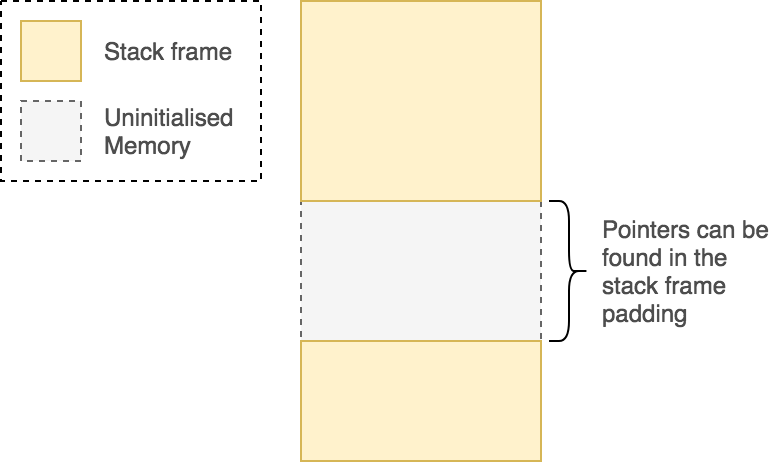
\includegraphics[max width=\linewidth]{figs/stackframepadding.png}
    \caption{A diagram showing the stack frame padding problem}
    \label{fig:stackframepadding}
\end{figure}

\section{Summary}

In this chapter I have discussed the implementation of each of the components of my garbage collector and how they work together to make the final solution. I have demonstrated how the Allocator manages the program's memory, maintains object meta-data which is used by the garbage collector and implements a write-barrier. Garbage collection details such as root finding, tracing and freeing garbage have all been discussed with pseudo-code given for the important functions. Finally, the multi-threaded extension has been discussed including how signal handlers have been used to implement a stop-the-world garbage collector. In the next section I will demonstrate that this implementation has been successful through unit testing and the analysis of custom benchmarks.

\end{document}